\documentclass{beamer}
\usepackage{beamerthemesplit}
\usepackage{wrapfig}
\usetheme{SPbGU}
\usepackage{pdfpages}
\usepackage{cmap} 
\usepackage{indentfirst}
\usepackage{multirow}
\usepackage[noend]{algpseudocode}
\usepackage{algorithm}
\usepackage{algorithmicx}
% \usetikzlibrary{shapes,arrows}
\usepackage{fancyvrb}
\newtheorem{rutheorem}{Теорема}
\newtheorem{ruproof}{Доказательство}
\newtheorem{rudefinition}{Определение}
\newtheorem{rulemma}{Лемма}
\beamertemplatenavigationsymbolsempty

\usepackage[utf8]{inputenc}
\usepackage[T2A]{fontenc} 
\usepackage[russian]{babel}
\usepackage{amsmath}
\usepackage{comment}

\usepackage{tikz}
\usepackage{graphicx}
\graphicspath{{../src/}}
\DeclareGraphicsExtensions{.png}

\renewcommand{\l}{\left( }
\renewcommand{\r}{\right) }
\renewcommand{\phi}{\varphi}
\newcommand{\pd}{\partial}
\newcommand{\br}[1]{\l {#1} \r}
\newcommand{\rint}{\int\limits_{-\infty}^{+\infty}}
\newcommand{\pint}{\int\limits_{-\pi}^{\pi}}
\newcommand{\jacobian}[2]{\frac{\pd \br{#1}}{\pd \br{#2}}}
\newcommand{\abs}[1]{\left| #1 \right|}


\title[]{Двухчастичные корреляции, возникающие при распаде одиночной струны}
% \subtitle[]{Опциональный подзаголовок}
% То, что в квадратных скобках, отображается в левом нижнем углу. 
\institute[СПбГУ]{
Санкт-Петербургский государственный университет \\
Кафедра физики высоких энергий и элементарных частиц }

% То, что в квадратных скобках, отображается в левом нижнем углу.
\author[Кравцов Павел]{Кравцов Павел Сергеевич, 408 группа \\
  % У научного руководителя должна быть указана научная степень
  \and  
    {\bfseries Научный руководитель:} д.ф.-м.н., профессор Вечернин В. В. \\ 
  % Для курсовой не обязателен. Должна быть указана должность или ученая степень
  \and
    {\bfseries Рецензент:} к.ф.-м.н., ассистент Алцыбеев И. Г.}

\date{6 июня 2016г.}

\definecolor{orange}{RGB}{179,36,31}

\begin{document}
\begin{comment}
\end{comment}
% титульный лист
{\begin{frame}
  \begin{center}
  {
\includegraphics[width=1.5cm]{SPbGU_Logo.png}}
  \end{center}
  \titlepage
\end{frame}}

% цель работы
\begin{frame}[fragile]
    \frametitle{Цель работы}
    
    \begin{minipage}[h]{0.48\linewidth}
    \begin{figure}
    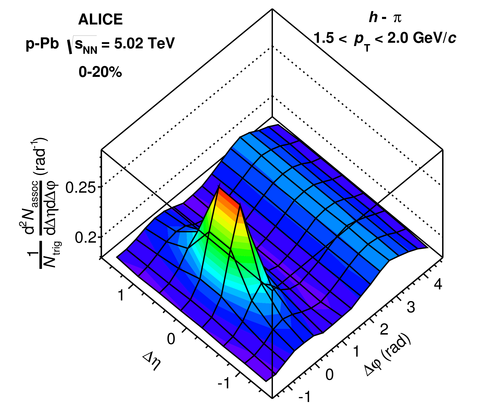
\includegraphics[width=\linewidth]{main.png}
    \caption{Распределение по разности быстрот $\Delta \eta$ и углу разлета $\Delta \phi$ частиц в процессе множественного рождения. График из \cite{exp_data}}
    \label{main}
    \end{figure}
    \end{minipage}
    \hfill
    \begin{minipage}[h]{0.48\linewidth}
    {\bfseries Цель работы: \\}
    Объяснить задний хребет на рис.~\ref{main}. \\
    \vfill
    $\Delta \eta$ - разноть быстрот частиц \\
    $\Delta \phi$ - угол разлета (угол между поперечными импульсами частиц) \\
    \vfill
    Определение быстроты:
    \begin{gather}
    \eta = ln \frac{1 + V_z}{1 - V_z},
    \end{gather}
    где $V_z$ - продольная скорость частицы.
    \end{minipage}
\end{frame}

% модель кварк-глюонной струны
\begin{frame}[fragile]
    \frametitle{Модель кварк-глюонной струны}
    
    \begin{itemize}
    \item Двухстадийное описание столкновений адронов
    \item Модель "yo-yo" струны
    \item Механизм фрагментации струны
    \end{itemize}
\end{frame}

% Двухстадийное описание столкновений адронов
\begin{frame}[fragile]
    \frametitle{Двухстадийное описание столкновений адронов}
    \begin{center}
    \begin{minipage}[h]{0.18\linewidth}
    \end{minipage}
    \hfill
    \begin{minipage}[h]{0.8\linewidth}
    \begin{tikzpicture}
    % Адроны
    \draw[thick] (-3,0) circle (1);
    \draw[->] (-2,0) -- (-.5, 0) node[below left] {$\eta$};
    \draw[thick] (3,0) circle (1);
    \draw[->] (2,0) -- (.5, 0) node[below right] {$\eta$};
    % кварки
    \draw[very thick] (-3, 0) +(90: .5)  coordinate (Q1) circle (0.3);
    \draw[very thick] (-3, 0) +(210: .5) coordinate (Q2) circle (0.3);
    \draw[very thick] (-3, 0) +(-30: .5) coordinate (Q3) circle (0.3);
    \draw[very thick] ( 3, 0) +(90: .5)  coordinate (Q4) circle (0.3);
    \draw[very thick] ( 3, 0) +(210: .5) coordinate (Q5) circle (0.3);
    \draw[very thick] ( 3, 0) +(-30: .5) coordinate (Q6) circle (0.3);
    
    % подписи
    \draw (-3, 1) node[above] {адрон};
    \draw (3, 1) node[above] {адрон};
    \draw[thin] (-3.5, -1) node[below] {кварки} -- (Q2) (-3.5, -1) -- (Q3);    
    \end{tikzpicture}
    \end{minipage}
    \vfill
    
    \begin{minipage}[h]{0.18\linewidth}
    \Huge 1
    \end{minipage}
    \hfill
    \begin{minipage}[h]{0.8\linewidth}
    \begin{tikzpicture}
    % Адроны
    \draw[thick] (-3,0) circle (1);
    \draw[thick] (3,0) circle (1);
    % кварки
    \draw[very thick] (-3, 0) +(90: .5)  coordinate (Q1) circle (0.3);
    \draw[very thick] (-3, 0) +(210: .5) coordinate (Q2) circle (0.3);
    \draw[very thick] (-3, 0) +(-30: .5) coordinate (Q3) circle (0.3);
    \draw[very thick] ( 3, 0) +(-90: .5)  coordinate (Q4) circle (0.3);
    \draw[very thick] ( 3, 0) +(-210: .5) coordinate (Q5) circle (0.3);
    \draw[very thick] ( 3, 0) +(30: .5) coordinate (Q6) circle (0.3);
    
    % струны
    \draw[thick, dashed] (Q1) +(90: .4) coordinate (A1) arc (90:270:0.4) coordinate (A3);
    \draw[thick, dashed] (Q4) +(90: .4) coordinate (A2) arc (90:-90:0.4) coordinate (A4);
    \draw[thick, dashed] (A1) -- (A2) (A3) -- (A4);
    
    \draw[thick, dashed] (Q2) +(90: .4) coordinate (A5) arc (90:270:0.4) coordinate (A6);
    \draw[thick, dashed] (A5) -- +(1.5, 0) coordinate (B1) (A6) -- +(1.5, 0) coordinate(B2);
     \draw[thick, dashed] (Q6) +(90: .4) coordinate (A7) arc (90:-90:0.4) coordinate (A8);
    \draw[thick, dashed] (A7) -- +(-1.5, 0) coordinate (B3) (A8) -- +(-1.5, 0) coordinate(B4);
    \draw[thick, dashed] (B1) -- (B3) (B2) -- (B4);
    \draw[thin] (0, -1) node[below] {струны} -- (.5,0) (0, -1) -- (-.5, 0); 
    \end{tikzpicture}
    \end{minipage}
    \vfill
    
    \begin{minipage}[h]{0.18\linewidth}
    \Huge 2
    \end{minipage}
    \hfill
    \begin{minipage}[h]{0.8\linewidth}
    \begin{tikzpicture}
    \draw[very thick] (-3, 0) coordinate (Q1) circle (0.3);
    \draw[very thick] ( 3, 0) coordinate (Q2) circle (0.3);
    \draw[thick] (Q1) +(90: .4) coordinate (A1) arc (90:270:0.4) coordinate (A3);
    \draw[thick] (Q2) +(90: .4) coordinate (A2) arc (90:-90:0.4) coordinate (A4);
    \draw[thick] (A1) -- (A2) (A3) -- (A4);
    \draw[->] (Q1) +(-0.4, 0) -- +(-1,0);
    \draw[->] (Q2) +( 0.4, 0) -- +( 1,0);
    \draw[thick] (1.5, 0) circle (0.4);
    \draw[thick, dashed] (1.7, 0) circle (0.4);
    \draw[thick] (-1.5, 0) circle (0.4);
    \draw[thick, dashed] (-1.3, 0) circle (0.4);
    
    \end{tikzpicture}
    \end{minipage}    
    \end{center}
 
\end{frame}

% yo-yo
\begin{frame}[fragile]
    \frametitle{"Yo-yo" струна}
    \begin{center}
    ${\tiny
    S = \gamma \int d\sigma \int d\tau \sqrt{\br{\frac{\pd x_\mu}{\pd \tau} \frac{\pd x^\mu}{\pd \sigma}}^2 - \br{\frac{\pd x_\mu}{\pd \sigma} \frac{\pd x^\mu}{\pd \sigma}} \br{\frac{\pd x_\nu}{\pd \tau} \frac{\pd x^\nu}{\pd \tau}}},
    }$
    \end{center}
    \begin{minipage}[h]{0.35\linewidth}
    {\small
    где $\gamma=const$ - натяжение струны, \\
    $\sigma, \tau$ - переменные, параметризуюшие струну, \\
    $x^\mu=x^\mu \br{\sigma, \tau}$ - координаты струны. \\
    $$$$
    $$$$
    $$$$
    }
    \end{minipage}
    \hfill
    \begin{minipage}{0.63\linewidth}
    \begin{figure}
    \center{
    \begin{tikzpicture}[scale=0.6]
    % оси координат
    \draw[->] (-2, 0) coordinate (O) -- +(5, 0) node [right] {$z$};
    \draw[->] (O) -- +(0, 7) node [left] {$t$};
    % пунктирные прямые
    \draw[thick, dashed]
    (0, 0) coordinate (A) -- +(-45:.5) 
    (0, 0) -- +(-135:.5)
    (0, 0) -- ++(45:3) -- ++(135:2) coordinate (B) -- ++(225:3) -- +(315:2) ++(45:3)
    -- ++(45:3) -- ++(135:2) coordinate (C) -- ++(225:3) -- +(315:2) ++(45:3)
     -- +(45:.5) 
     +(0,0) -- +(135:.5);
    % гиперболы
     \draw[thick]
    (A) .. controls +(50:2.8) .. (B)
    (A) .. controls +(130:1.85) .. (B)
    (B) .. controls +(50:2.8) .. (C)
    (B) .. controls +(130:1.85) .. (C)
    (A) -- +(-55:.4)
    (A) -- +(-125:.4)
    (C) -- +(125:.4)
    (C) -- +(55:.4);
    \end{tikzpicture}
    }
    \caption{Движение концов струны "yo-yo" с массами (сплошная линия) и без масс (пунктирная линия).}
    \label{yoyo}
    \end{figure}
    \end{minipage}
\end{frame}

% fragmentation
\begin{frame}[fragile]
\frametitle{Механизм фрагментации струны}
\begin{minipage}[h]{0.48\linewidth}
\begin{figure}
\center{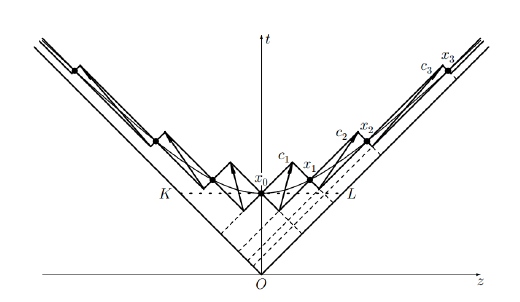
\includegraphics[width=0.8\textwidth]{fragmentation.png}}
\caption{Доминирующий процесс фрагментации струны. 
Все разрывы происходят с $S = S_0$. 
Иллюстрация из \cite{fragmentation_lit}}
\label{fragmentation}
\end{figure}
\end{minipage}
\hfill
\begin{minipage}[h]{0.48\linewidth}
\begin{gather}
dP \br{S} = \frac{1}{S_0} \br{1 - P \br{S}} dS, \nonumber
\end{gather}
где $S_0$ - параметр модели.
\begin{gather}
P \br{S} = 1 - exp \br{-\frac{S}{S_0}} \nonumber
\end{gather}
$$$$
\center{\fbox{$\abs{\Delta \eta} \approx 1$}}
\end{minipage}
\end{frame}

% обзор по струнам
\begin{frame}[fragile]
\frametitle{Источники и виды корреляций}
\begin{enumerate}
\item Дальние корреляции
    \begin{itemize}
    \item Флуктуация числа струн-источников
    \item Слияние струн 
    \end{itemize}
\item Ближние корреляции
    \begin{itemize}
    \item Локальные законы сохранения
    \end{itemize}
\end{enumerate}
\end{frame}

% single string model
\begin{frame}[fragile]
\frametitle{Модель одиночной струны}
\begin{figure}
\center{
\begin{tikzpicture}[scale=0.5]
% оси X, Y, Z
\fill (1, 2) coordinate (O);
\draw[thick, ->] (O) node [below] {$O$} -- +(90:1) node [right] {$x$};
\draw[thick, ->] (O) node [below] {$O$} -- +(225:.5) node [left] {$y$};
\draw[thick, ->] (O) node [below] {$O$} -- +(0:1) node [right] {$z$};

%труба
\draw[very thick, gray] (0, .5) -- ++(1.5, 0) ++(1.5, 0) -- ++(9, 0) ++(1.5, 0) -- ++(1.5, 0);
\draw[very thick, gray, dashed] (1.5, .5) -- ++(1.5, 0) ++(9, 0) -- ++(1.5, 0);
\draw[very thick, gray] (0, -.5) -- ++(1.5, 0) ++(1.5, 0) -- ++(9, 0) ++(1.5, 0) -- ++(1.5, 0);
\draw[very thick, gray, dashed] (1.5, -.5) -- ++(1.5, 0) ++(9, 0) -- ++(1.5, 0);
\draw[very thick, gray] (0, .5) arc (90:270:0.25 and 0.5);
\draw[very thick, gray, densely dashed] (0, -.5) arc (270:450:0.25 and 0.5);
\draw[very thick, gray] (15, 0) ellipse (0.25 and 0.5);

% палочки между кварками
\draw[ultra thick]
(0.7, 0) coordinate (QM) -- +(-5:0.85)
(4.5, -.2) coordinate (AQ1) -- +(177:1.6)
(4.5, .2) coordinate (Q1) -- (7.5, .3) coordinate (AQ2)
(7.5, -.3) coordinate (Q2) -- (10.5, .2) coordinate (AQ3)
(10.5, -.2) coordinate (Q3) -- +(4:1.5)
(14.55, 0) coordinate(AQN) -- +(176:1.1) ;

% стрелочки
\def\impangle{40}
\draw[thick, ->] (Q1) -- +(\impangle :1.5) node [right] {$\vec{q_1}$};
\draw[thick, ->] (AQ1) -- +(\impangle + 180:1.5) node [left] {$\vec{\bar{q_1}}$};
\draw ++(Q1) -- +(90:1) +(\impangle:.5) arc (\impangle:90:.5) node [above right] {$\phi_1$};
\def\impangle{-70}
\draw[thick, ->] (Q2) -- +(\impangle :1.0) node [right] {$\vec{q_2}$};
\draw[thick, ->] (AQ2) -- +(\impangle + 180:1.0) node [above] {$\vec{\bar{q_2}}$};
\draw ++(Q2) -- +(90:1) +(\impangle:.5) arc (\impangle:90:.5) node [right] {$\ \phi_2$};
\def\impangle{-30}
\draw[thick, ->] (Q3) -- +(\impangle :2.0) node [right] {$\vec{q_3}$};
\draw[thick, ->] (AQ3) -- +(\impangle + 180:2.0) node [left] {$\vec{\bar{q_3}}$};
\draw ++(Q3) -- +(90:1) +(\impangle:.5) arc (\impangle:90:.5) node [right] {$\ \phi_3$};

% кварки
\draw[fill=gray] (QM) circle (0.15) node [left] {$\vec{q}_{-m}$};
\draw[fill=white] (AQ1) circle (0.15);
\draw[fill=gray] (Q1) circle (0.15);
\draw[fill=white] (AQ2) circle (0.15);
\draw[fill=gray] (Q2) circle (0.15);
\draw[fill=white] (AQ3) circle (0.15);
\draw[fill=gray] (Q3) circle (0.15);
\draw[fill=white] (AQN) circle (0.15) node [right] {$\ \vec{\bar{q_n}}$};
\end{tikzpicture}
}
\caption{Модель цветной кварк-глюонной струны}
\label{string}
\end{figure}
\begin{minipage}[h]{0.48\linewidth}
Дано:
\begin{itemize}
\item $\abs{\Delta \eta} = 1$
\item $\vec{p_i} = \vec{q}_{i+1} + \vec{\bar{q_i}} = \vec{q}_{i+1} - \vec{q_i}$
\item $\Delta \phi_i$ - угол между $p_i$ и $p_{i+1}$
\item $\rho_{\phi_i} \br{\phi_i} = \frac{1}{2 \pi}$
\item $\rho_{q_i} \br{q_i}$ известно
\end{itemize}
\end{minipage}
\begin{minipage}[h]{0.48\linewidth}
Найти:
\begin{itemize}
\item $\rho_{p_i} \br{p_i} = ?$
\item $\rho_{\Delta \phi_i} \br{\Delta \phi_i} = ?$
\end{itemize}
$$$$
$$$$
$$$$
\end{minipage}
\end{frame}

% const
\begin{frame}[fragile]
\frametitle{Константный случай}
\begin{minipage}[h]{0.48\linewidth}
Распределение импульсов кварков
$$\rho_{q_i} \br{q} = \delta \br{q - q_0}$$
$$$$
$$$$
Распределение импульсов мезонов
$$\rho_p \br{p} = \frac{2}{\pi\sqrt{\br{2 q_0}^2 -p^2}}$$
Распределение по углу разлета
$$\rho_{\Delta \phi} \br{\Delta \phi} = \frac{\abs{\Delta \phi}}{\pi^2}, \Delta \phi \in \left[ -\pi, \pi \right]$$
\end{minipage}
\begin{minipage}[h]{0.48\linewidth}
\center{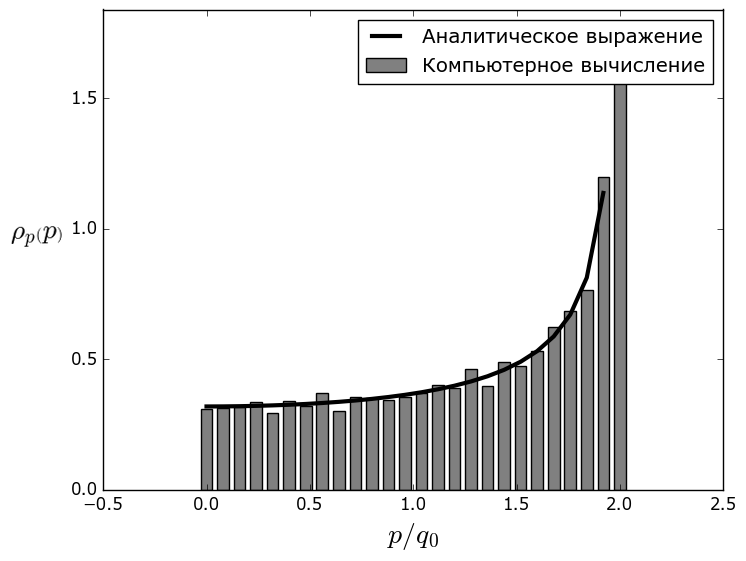
\includegraphics[width=0.9\linewidth]{const_momentum_10000}}
\center{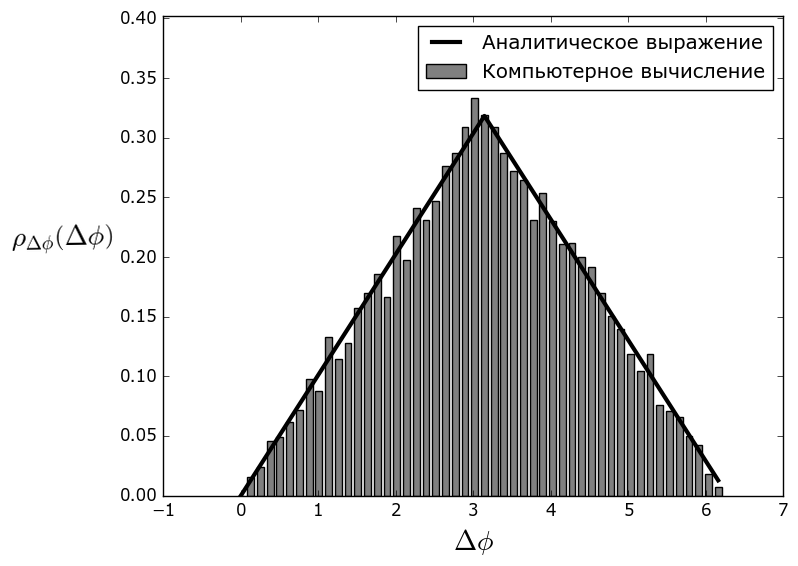
\includegraphics[width=0.9\linewidth]{const_alpha_10000}}
\end{minipage}
\end{frame}

% gauss
\begin{frame}[fragile]
\frametitle{Гауссов случай}
\begin{minipage}[h]{0.53\linewidth}
Распределение импульсов кварков
$$\rho_{q_i} \br{q} = \frac{q}{2 q_0^2} exp \br{-\frac{q^2}{q_0^2} }$$
$$$$
Распределение импульсов мезонов
$$\rho_p \br{p} = \frac{p \ e^{-\frac{p^2}{2q_0^2}}}{q_0^2} $$
Распределение по углу разлета \\
{\small
$\rho_{\Delta \phi} \br{\Delta \phi} = \frac{3}{8 \pi} \frac{\sqrt{1 - \br{\gamma / 2}^2} - \br{\gamma / 2} \ arccos \br{\gamma / 2}}{\br{1 - \br{\gamma/2}^2}^{3/2}},$ \\
$\quad \text{где} \ \gamma = cos \Delta \phi $
}
\end{minipage}
\begin{minipage}[h]{0.43\linewidth}
\center{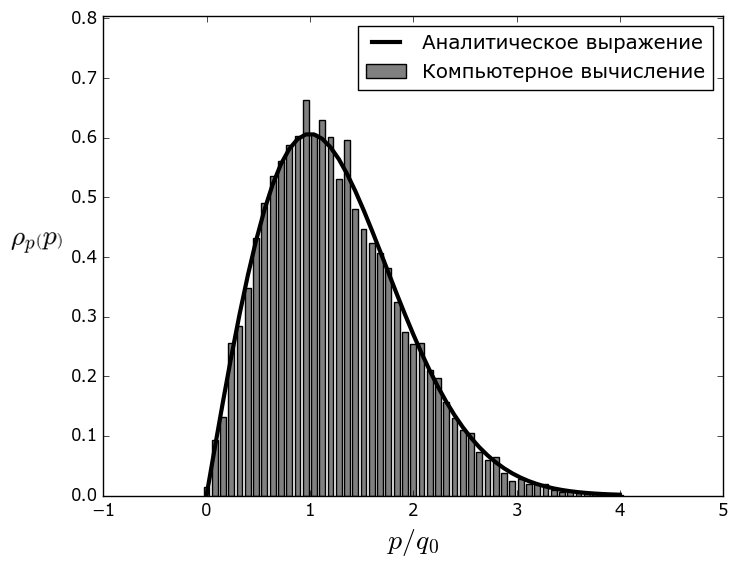
\includegraphics[width=1\linewidth]{gauss_momentum_10000}}
\center{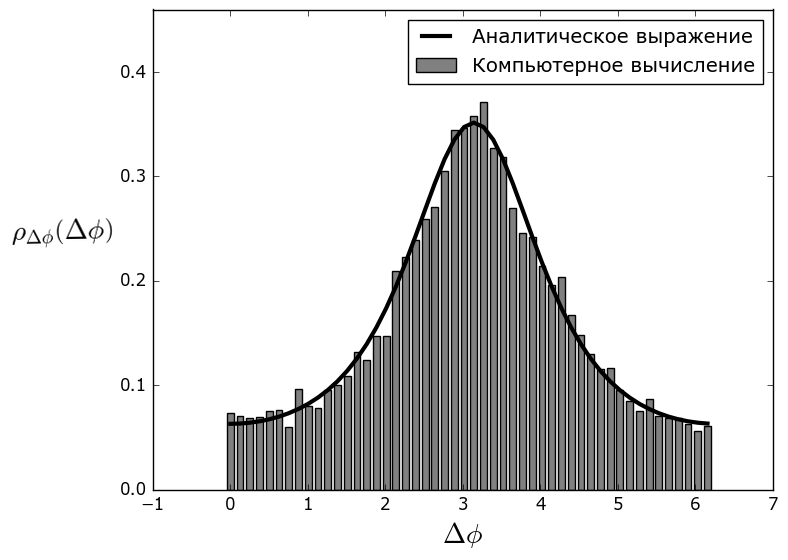
\includegraphics[width=1\linewidth]{gauss_alpha_10000}}
\end{minipage}
\end{frame}

% % корреляционная функция
% \begin{frame}[fragile]
% \frametitle{Импульсная корреляционная функция}
% Как правило:
% $$G^2 = G^2 \br{p_1^x, p_1^y, p_1^z, p_2^x, p_2^y, p_2^z}$$
% В работе:
% $$G^2 = G^2 \br{p_1, p_2, \phi_1, \phi_2, \eta_1, \eta_2} =$$ \\
% $$ = C_1 \cdot \frac{4}{3 \pi q_0^4}  p_1 p_2 \ exp \br{-\frac{2}{3q_0^2}\br{p_1^2 + p_2^2 + p_1 p_2 cos \br{\Delta \phi}}} \cdot$$
% $$\cdot \frac{ \delta \br{\Delta \eta - 1} + \delta \br{\Delta \eta + 1}}{2} + $$
% $$+ C_2 \cdot \rho_p \br{p_1} \cdot \rho_p \br{p_2} \cdot \rho_{\phi} \br{\phi_2} \cdot \rho_{\phi} \br{\phi_1} \cdot \rho_\eta \br{\eta_1} \cdot \rho_\eta \br{\eta_2}$$
% \end{frame}

% \begin{frame}[fragile]
% \frametitle{Импульсная корреляционная функция}
% Как правило:
% $$G^2 = G^2 \br{p_1^x, p_1^y, p_1^z, p_2^x, p_2^y, p_2^z}$$
% В работе:
% $$G^2 = G^2 \br{p_1, p_2, \phi_1, \phi_2, \eta_1, \eta_2} =$$ \\
% $$= \rho_p \br{p_1} \cdot \rho_p \br{p_2} \cdot \rho_{\Delta \phi} \br{\phi_2 - \phi_1} \cdot \rho_\eta \br{\eta_1} \cdot \rho_\eta \br{\eta_2}$$
% Можно считать, что 
% $$\rho_\eta = 
% \begin{cases}
% \frac{1}{\eta_{max} - \eta_{min}}, \text{если} \ \eta \in \left[ \eta_{min}, \eta_{max}\right] \\
% 0, \text{иначе}
% \end{cases}$$
% \end{frame}

% Объяснение заднего хребта
\begin{frame}[fragile]
\frametitle{Объяснение наличия заднего риджа}
\begin{minipage}[h]{0.48\linewidth}
\begin{figure}
\center{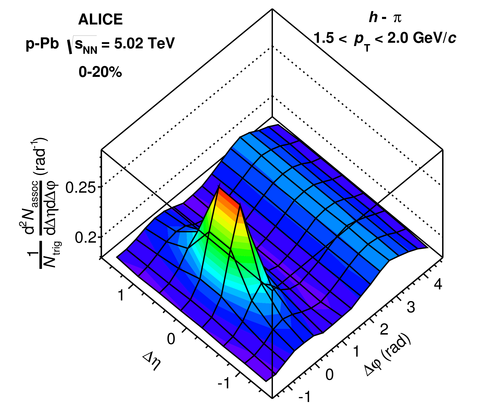
\includegraphics[width=1\textwidth]{main.png}}
\caption{Экспирементальное распределение числа частиц по $\br{\Delta \eta, \Delta \phi}$  }
\end{figure}
\end{minipage}
\begin{minipage}[h]{0.48\linewidth}
\begin{figure}
\center{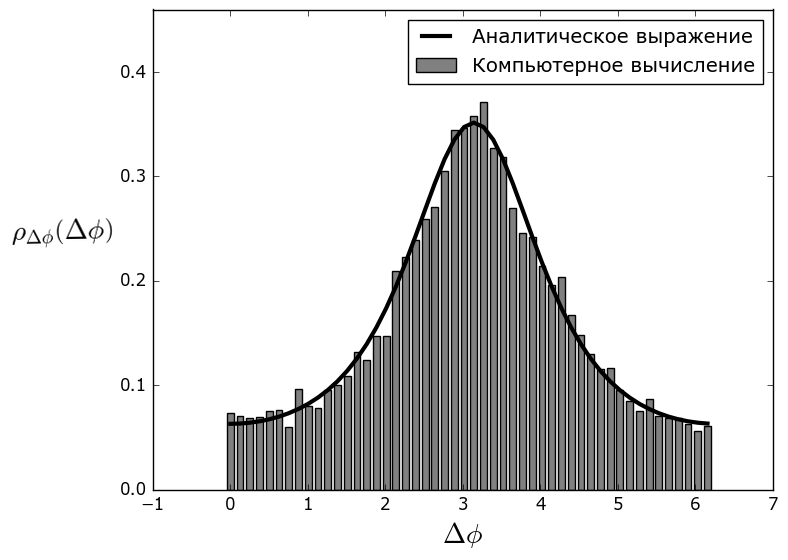
\includegraphics[width=0.8\linewidth]{gauss_alpha_10000}}
\end{figure}
\center{Модель предсказывает:}
\begin{figure}
\center{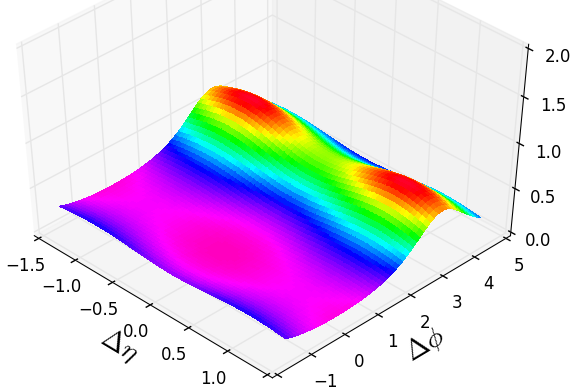
\includegraphics[width=0.8\linewidth]{must_be}}
\end{figure}
\end{minipage}
\end{frame}

% результаты
\begin{frame}[fragile]
\frametitle{Результаты}
\begin{itemize}
% \item Построена импульсная корреляционная функция для модели одиночной струны
\item В рамках модели объяснен задний хребет
\item Построенную модель можно использовать в монте-карловских генераторах событий
\end{itemize}
\end{frame}

%literature 1
\begin{frame}[fragile]
\frametitle{Список литературы\footnote{Использован стилевой файл презентации из репозитория github.com/YaccConstructor/articles/tree/master/SlidesTemplate
}}
{\small
\begin{thebibliography}{00}
\bibitem{model1}
A. B. Kaidalov, Phys. Lett. B 116, p.459 (1982).
\bibitem{model2}
A. B. Kaidalov, K. A. Ter-Martirosyan, Phys. Lett. B 117 p.247 (1982).
\bibitem{model3}
A. Cappela, U. Sukhatme, Chung-I Tan, J. Tran Thanh Van, Phys. Lett. B 81, 68 (1979).
\bibitem{model4}
A. Cappela, U. Sukhatme, Chung-I Tan, J. Tran Thanh Van, Phys. Rep. 236 p.225 (1994).
\bibitem{nesterenko}
Барбашов Б. М., Нестеренко В. В. Модель релятивистской струны в физике адронов, М.: Энергоиздат, 1987.
\bibitem{schwinger}
J. Schwinger, Phys. Rev. 82, p.664 (1951).
\bibitem{artru}
X. Artru, Phys. Rep. 97, p.147 (1983).
\bibitem{fragmentation_lit}
V. V. Vechernin, arXiv: 0812.0604 [hep-ph].
\end{thebibliography}
}
\end{frame}

%literature 2
\begin{frame}[fragile]
\frametitle{Список литературы}
{\small
\begin{thebibliography}{00}
\bibitem{cappela}
A. Capella, A. Krzywicki, Phys. Rev. D 18 p.4120 (1978).
\bibitem{exp_data}
{\bf ALICE} Collaboration, B. Abelev \textit{et al.}, arxiv:1307.3237 [nucl-ex].
\bibitem{fusion1}
M. A. Braun, C. Pajares, Phys. Lett. B 287, p.154 (1992).
\bibitem{fusion2}
M. A. Braun, C. Pajares, Nucl. Phys. B 390, p.542 (1993).
\bibitem{fusion_corr1}
N. S. Amelin, N. Armesto, M. A. Brown, E. G. Ferreiro, C. Pajares, Phys. Rev. Lett. 73, p.2813 (1994).
\bibitem{fusion_corr2}
M. A. Braun, R. S. Kolevatov, C. Pajares, V. V. Vechernin, Eur.Phys. J. C 32, p.535 (2004); arXiv:hep-ph/0307056.
\bibitem{fusion_corr3}
V. V. Vechernin, R. S. Kolevatov, Phys. Atom. Nucl. 70 p.1797 (2007).
\bibitem{fusion_corr4}
V. V. Vechernin, R. S. Kolevatov, Phys. Atom. Nucl. 70 p.1809 (2007).
\bibitem{venus}
K. Werner, Phys. Rep. 232, p.87 (1993).
\end{thebibliography}
}
\end{frame}
\end{document}
